\vspace{-3mm}
\section{Requirements}	

	\normalsize
	{		
		The elicitation of requirements can be obtained from many different techniques.
		The categorisation of requirements capture methods according to \citet{Goguen} can be divided into 4 main categories,
		traditional, cognitive, collaborative \& contextual techniques.	

		\vspace{-3mm}
		\begin{multicols}{2}
		
			\begin{itemize}
				\item \textbf{Traditional} 
					\newline
					including introspection, reading existing documents, analysing data,
					interviews, surveys \& questionnaires and meetings.
				\item \textbf{Cognitive}	
					\newline
					including task analysis, protocol analysis \& knowledge acquisition techniques.
		
		\vfill
		\columnbreak
		
				\item \textbf{Collaborative}	
					\newline
					including group techniques, workshops, prototyping \& participatory design.					
				\item \textbf{Contextual}	
					\newline
					including ethnographic analysis, discourse analysis \& sociotechnical methods.
					\newline
			\end{itemize}
		
		\end{multicols}	

		\textit{Those who have completed human computer interaction studies will be familiar with these techniques.
		These techniques are outside the scope of this report and I ask the reader to refer to Jakob Neilson 
		and his usability books series, which describe these techniques in detail.}
		\newline
		\newline
		Although no one categorisation was used in the elicitation of the requirements, there was a particular affinity
		to the cognitive category.  I, having previous experience in the role of Unix Systems Administrator in multi nationals corporations,
		identified with the repetitive processes in place in these companies. The tasks, protocol compliance and knowledge acquisition  
		incepted the concept and the key requirements of this project.  The following marchitecture (or marketecture) presents the key requirement artefacts.		
	}
	
	\vspace{3mm}
	\noindent\begin{minipage}{\textwidth}
			
		\begin{figurehere}
			\centering
			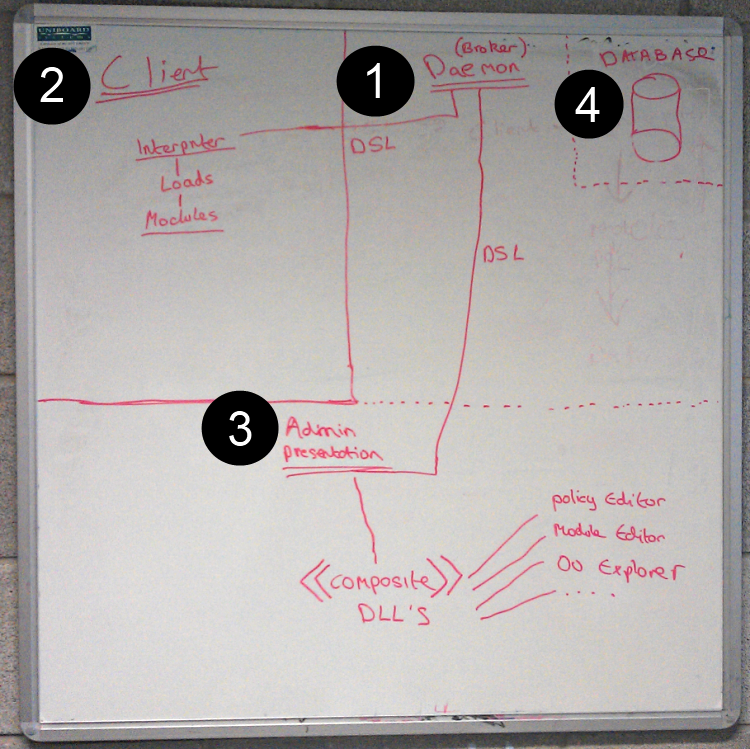
\includegraphics[scale=0.45]{pages/chapter3/figures/march2.png}
			\vspace{-2mm}
			\caption{Marchitecture}
			\label{fig:Marchiteture}
		\end{figurehere}	
	
	\end{minipage}	
		
	\vspace{3mm}
	\normalsize
	{
		To begin to understand the requirements and the resulting implementation,  Fig. \ref{fig:Marchiteture} 
		presents a marchitecture of a high level architectural design.  
		The marchitecture indicates the four main artefacts that support the requirements.
		
		\vspace{-3mm}
		\begin{multicols}{2}
		
			\begin{enumerate}[itemsep=0pt,parsep=0pt]

				\item \textbf{Daemon (Broker - Server)} 
					\begin{itemize}
						\item Broker between the admin presentation and the clients 
					\end{itemize}	
					
				\item \textbf{Client} 
					\begin{itemize}
						\item Interpreter which parses the domain specific language (DSL)
						\item Interpreter which loads modules to extend the parsing (rules) capabilities of the interpreter.
					\end{itemize}

			\columnbreak
					
				\item \textbf{Admin Presentation}	
					\begin{itemize}
						\item Linux Group Policy Administrator interface 
						\item Composite architecture
						\item Creates rules in the form of a domain specific language (DSL)
					\end{itemize}	
					
				\item \textbf{Database} 
					\begin{itemize}
						\item Ultimately stores all domain specific data
						\item Policies ( domain specific language )
					\end{itemize}	
					
			\end{enumerate}		
			
		\end{multicols}
		\vspace{-1mm}
		
		A recurring artefact here is the domain specific language (DSL). So I will provide a fifth section
		
		\begin{enumerate}
			\setcounter{enumi}{4}
			\item \textbf{Domain Specific Language (DSL)} 
				\vspace{-2mm}
				\begin{itemize}
					\item How rules are specified through a domain specific language
				\end{itemize}			
		\end{enumerate}		
	}		
